\documentclass[11pt]{scrreprt}
\usepackage[sexy, titlemark]{evan}

\begin{document}
\title{Helium 2.0 User Manual}
\subtitle{Harvard-MIT Math Tournament}
\author{Evan Chen}
\date{\today}
\maketitle

\begin{abstract}
	Helium is a grading system for math contests.
	It was developed for HMMT in October of 2016 following inspiration
	from the Stanford Math Tournament's new Atomic Grader.

	Helium is built using Django to be compatible with
	HMMT's then-existing structure.
	It features scan-based grading, a rapid-fire score input system,
	as well as support for direct score entry.
	Conflict resolution is handled automatically,
	as well as generating of results according to the
	HMMT scoring algorithm.
	The Django admin interface is built in.

	This documentation is split into several parts.
	Chapters are dedicated to graders (day-of volunteers),
	officers (trusted staff members with extra responsibilities),
	system administrators (with setup and result checking before the tournament),
	and finally other developers (who wish to play with code),
	with each section more technical and detailed than the last.

	The appendix consists of a list of terminology which
	will be used throughout the manual.
	Also, a note that screenshots may be slightly out of date.

	\begin{center}
		
\includegraphics[width=0.99\textwidth]{../img/balloons.png}
	\end{center}
\end{abstract}

\tableofcontents

\chapter{Instructions for Graders}
This details the tasks which should be performed by day-of graders.
Most graders will only need to read this chapter of the manual,
and maybe the terminology section (Appendix~\ref{ch:terms}).

The two functions that you care about are ``Grade Scans''
and ``Classical Grader''

\section{Scan grading}
This is pretty self-explanatory.

\begin{center}
	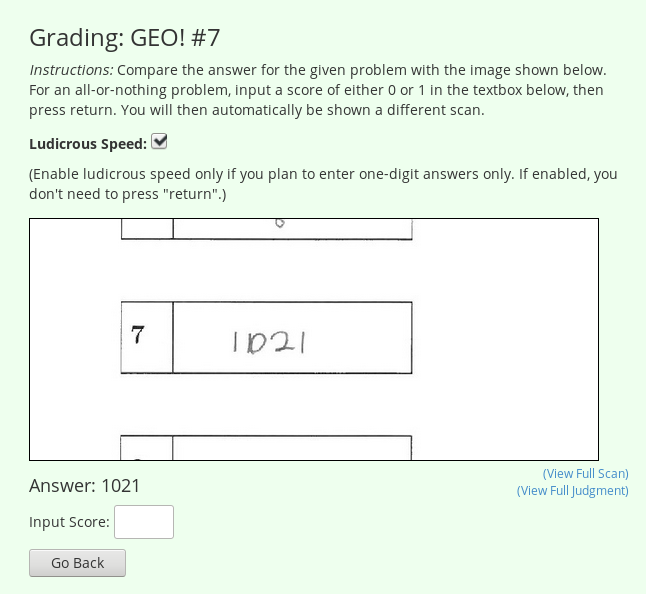
\includegraphics[width=0.8\textwidth]{images/scangrade.png}
\end{center}

%To do this, you should select a problem from the landing page,
%which will open the scan grader for that page.
\begin{itemize}
	\ii Try to select one of the $10$ problems from an exam at random,
	so that we don't end up with everyone problem $1$ or something.
	\ii For all-or-nothing problems,
	type $0$ for an incorrect answer and $1$ for a correct answer.
	\ii Press ``go back'' if you made a mistake and want to fix it.
\end{itemize}
It's possible that you might have some problems
where scores entered are not just $0$ or $1$.
That's fine too.

The option ``ludicrous speed'' is enabled by default (checkbox above),
as long as the problem you are grading is not all-or-nothing.
This means that you don't have to press enter.
If you prefer to take things more slowly,
or for some reason the problem you are grading accepts
scores other than $0$ or $1$,
you should disable this option.

If configured, the background of the page may be tinted
with the color of the test, so that you don't accidentally grade
the wrong test.

\section{Classical grader}
Most importantly:
\emph{do not use the classical grader on problems graded by scan}!
(The interface disables this by default.)

\begin{center}
	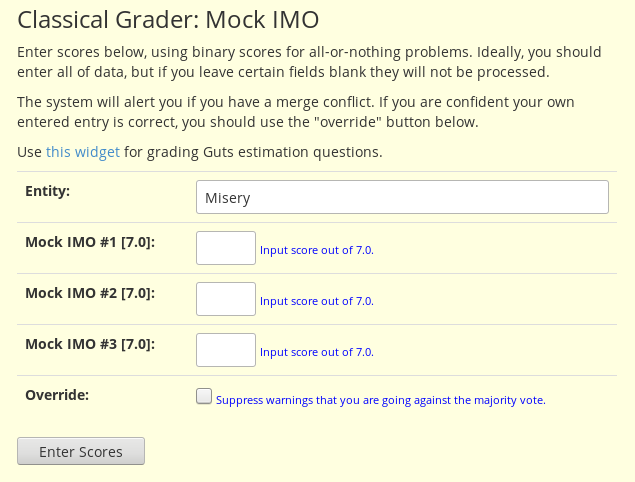
\includegraphics[width=0.8\textwidth]{images/classicgrade.png}
\end{center}

Use the classical grader for tests which are not graded by scan
(for example, the Guts round).
There are two ways you can do this:
\begin{itemize}
	\ii Grade by exam, meaning you are grading many problems on that exam.
	\ii Grade by problem, meaning that you are only grading 
	a particular problem (for example a February proof-based team round problem).
\end{itemize}
Afterwards, this is self-explanatory;
select the entity you want, enter their scores, and submit!

This time, Helium will warn you if you are submitting
a score that goes against a consensus for that problem
(for example if Alice enters 1 and then Bob tries to enter 0 later,
Helium will warn Bob).
If you are confident you are correct, you can use the override option.
However ideally when this happens you should find the person
who submitted the wrong answer before and check with them first.

Whenever you select an entity,
the scores you previously entered for that
entity will be automatically displayed.

If configured, the background of the page may be tinted
with the color of the test, so that you don't accidentally grade
the wrong test.

\section{Matching names}
The other option you can do, if you want something a little
less thoughtless than pressing the zero or one key,
is to help with matching students to names.
This feels quite similar to the scan grader,
but the difference is there are three options you can choose
for each scan.

\begin{center}
	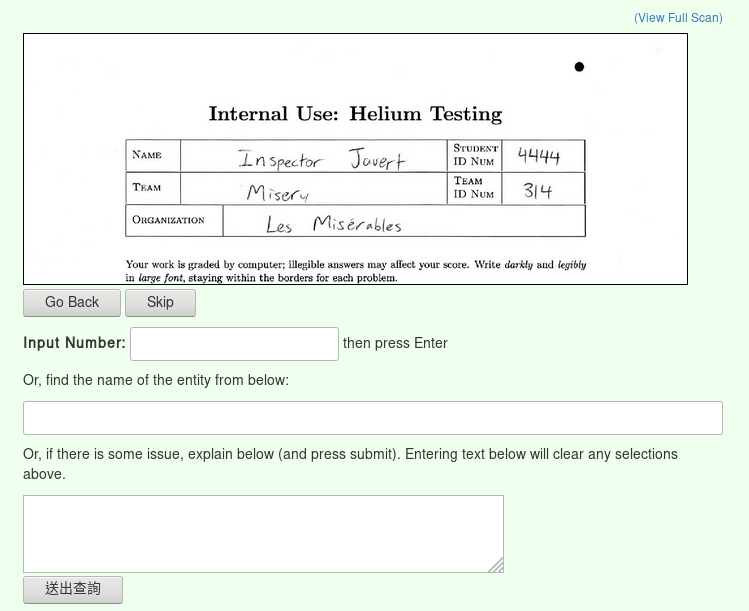
\includegraphics[width=0.7\textwidth]{images/fastmatch2.png}
\end{center}

There are three things you can do for each student name:
\begin{enumerate}
	\ii Most easily, input the student's ID number.
	Type in the student's number into the text box;
	the autocomplete field will then match with the name of the student.
	Press enter to submit.

	\ii Alternatively you can try searching by name.
	Type in the name in the autocomplete field;
	upon getting a match, select it and press enter.
	This works equally well.
	I think it's faster to use ID numbers when possible, but to each their own.

	\ii If their some other issue with the scan
	(e.g.\ there is no name or number at all,
	or the student doesn't appear to exist),
	you should flag it for administrative attention.
	To do this, simply fill in the text box, and press submit.
	An administrator will then be able to deal with it.
\end{enumerate}

\section{Viewing Full Scans}
\label{sec:view_full}
When doing scan grading, you can press ``view full page''
in order to see the entire scanned page instead of just the cut-out.
Just click the ``(View Full Scan)'' button near the corner of the image.

On this page there is also a switch where you can flag the page
for administrative attention, if there is something wrong with it
(for example, it is blank, or rotated, or illegible, etc.).

\section{Guts round}
\begin{itemize}
	\ii Guts round scoring is done using the classical grader.
	\ii For the ``estimation problems'' you will have to compute the score
	to assign to the problems at the end.
	So a ``Guts estimation calculator'', self-explanatory,
	has been provided.
	\ii The old Babbage Guts scoreboard should still be working
	(it now pulls data from Helium).
\end{itemize}

\section{Viewing conflicts}
You can see any evidences you submitted which conflicted with other graders
by pressing ``View Your Grading Conflicts''.
This allows you to also open any particular verdict,
and change your decision on it.

\begin{center}
	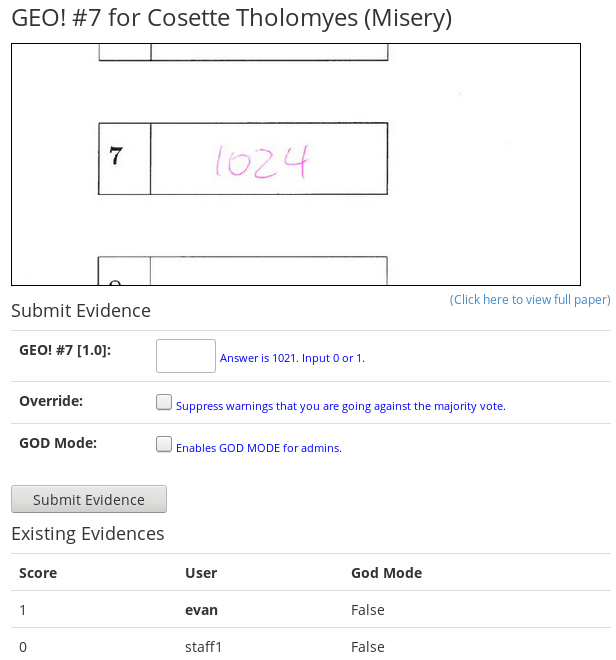
\includegraphics[width=0.7\textwidth]{images/viewverdict.png}
\end{center}
\begin{center}
	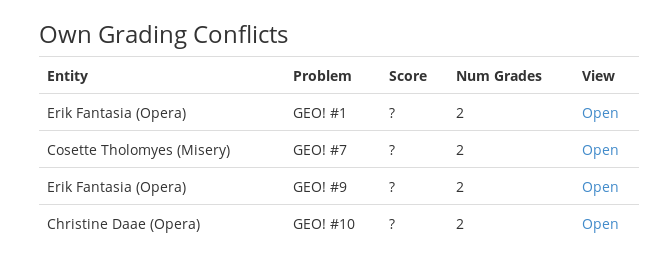
\includegraphics[width=0.8\textwidth]{images/viewconflict.png}
\end{center}

This shouldn't really be necessary for scan grading,
because verdicts are settled with a sufficiently large majority vote anyways.
That is, if you mis-grade a scan, it will eventually sort itself out.

\section{Progress grading}
There are some progress reports on how far grading is going for each problem.
You can use this if you're not sure which problems needs more help.
(Officers may also use this so they can panic as they see things aren't getting done,
or something like that.)

\begin{center}
	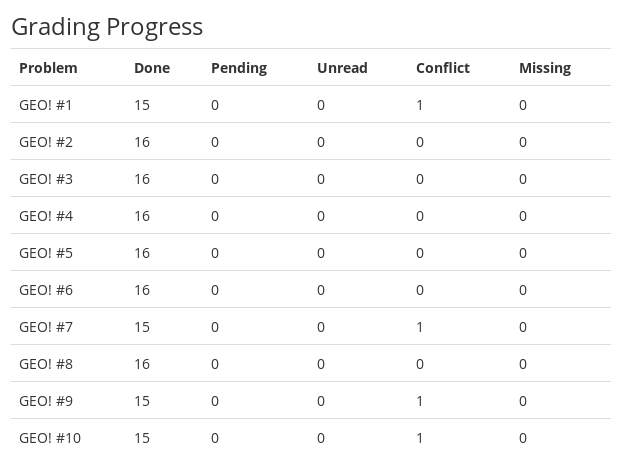
\includegraphics[width=0.8\textwidth]{images/progress.png}
\end{center}


\section{Sneak peek at results}
Some of you may be curious at how teams or students are doing.
While I can't endorse this, the interface lets you do so:
you can poke around the results page,
or look up student papers, etc.
If you do look through this, note that:
\begin{itemize}
	\ii Nothing you see is final, and
	\ii All results are confidential.
\end{itemize}
Note that results are not computed in realtime.
The algorithmic scoring always takes a few minutes.

\section{Do not use ``Upload Scans''}
Unless instructed to do so.

\chapter{Instructions for officers}
This assumes you have super-user privileges.
So it contains some higher-level administration tasks.

\section{Uploading scans}
Self-explanatory, but some gotchas:
\begin{itemize}
	\ii For safety, uploaded filenames \emph{must} be distinct.
	(This is to prevent someone from accidentally submitting the form twice,
	or submitting the same PDF twice.)
	If your scanner has silly filenames, fix those.
	Also, filenames should end with either ``pdf'' or ``PDF''.

	\ii At the moment we don't have image processing,
	so please make sure all scans are correctly rotated.

	\ii \emph{Please}, make sure you are uploading the scans
	to the correct contest!
	There are some ways to deal with such mistakes but better
	if they can be avoided in the first place.
\end{itemize}

\begin{center}
	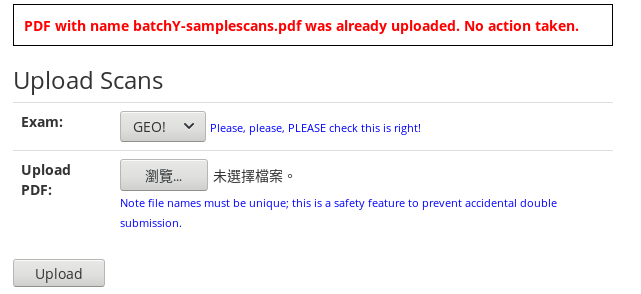
\includegraphics[width=0.8\textwidth]{images/batchscan.png}
\end{center}

When you upload a scan,
several problem scribbles, exam scribbles, and verdicts
are immediately created corresponding to the items in the PDF file.
However since the system does not yet know who is who,
the verdicts and problem scribbles will not have an entity attached to them.
The ``match scans'' functionality will then pair them up.

\section{Matching scans}
Matching scans is more error-prone and not double-checked.
People who should do this should be ones who are a little familiar with
all the teams attending and so on (e.g.\ TD's and registration director at HMMT).

\begin{center}
	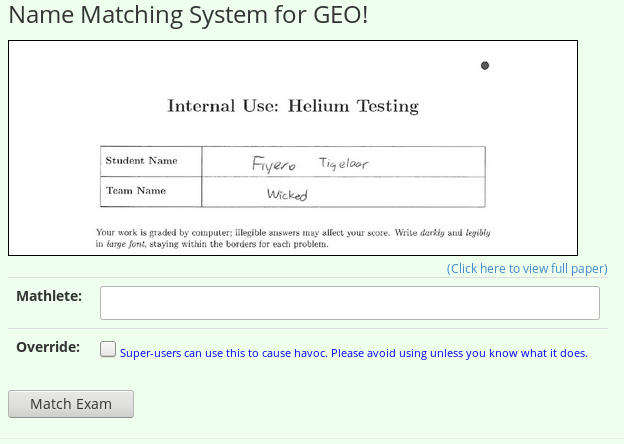
\includegraphics[width=0.8\textwidth]{images/papermatch.png}
\end{center}

Interface usage: a name will be shown.
\begin{itemize}
	\ii Find the corresponding entity, and submit.
	\ii If all goes well, next entity will be shown.
\end{itemize}
Easy.
When a match of a paper is successful,
all the problem scribbles, exam scribbles, and verdicts
attached to the paper are immediately updated to reflect the new name.

The comments in Section~\ref{sec:view_full} apply equally well here.

\subsection{Error handling}
This is where it gets tricky.
Consider the following situation:
\begin{quote}
	You match a geometry exam to a student ``Christine Daae''.  
	Later on, you try to match another geometry exam
	to the same student ``Christine Daae''.
\end{quote}
This is obviously not okay, and the system will complain.
An error will appear linking to the first \emph{verdict}
it finds for a geometry problem taken by Christine Daae.

\begin{center}
	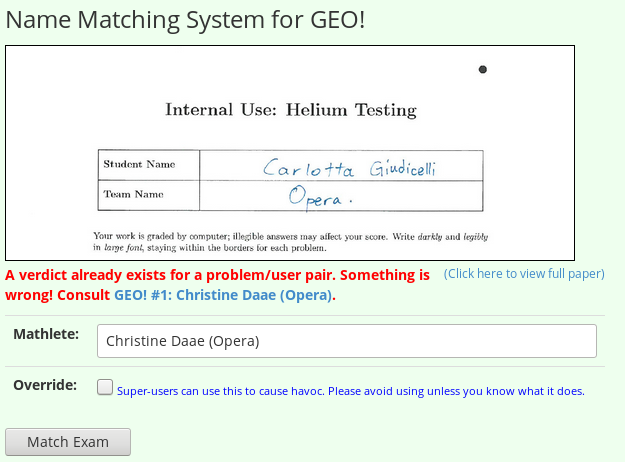
\includegraphics[width=0.7\textwidth]{images/matchconflict.png}
\end{center}

At this point you need to fix the error.
There are a couple things you could do.
\begin{itemize}
	\ii If you made the mistake this time,
	then just re-submit the form with the correct name. Easy.

	\ii If you made the mistake the \emph{first} time around,
	then you need to go back and fix it.

	You can do this by clicking on the verdict provided by the system,
	and then opening the exam scribble for that verdict.
	Alternatively, the ``Find Papers'' interface will let you find
	the previous paper as well.
	This will bring you to a match form where you can change the
	name to the correct one.

	\ii As a last resort,
	the ``Override'' switch (visible only to super-users)
	will forcibly assign the paper,
	and retroactively delete all verdicts and
	problems scribbles to the contrary.
	This is a Bad Idea\texttrademark\ and you should only do it
	if you really understand Helium well and have a compelling reason to do so.
\end{itemize}

\section{Find papers}
You can locate specific papers
by selecting ``Find Papers'' from the index page.
Some ways to do so:
\begin{itemize}
	\ii You can look up by exam and entity.
	\ii You can scroll through the pages of the PDF files.
	\ii A list of papers which need moderator attention
	will appear here (see Section~\ref{sec:view_full}).
\end{itemize}

\begin{center}
	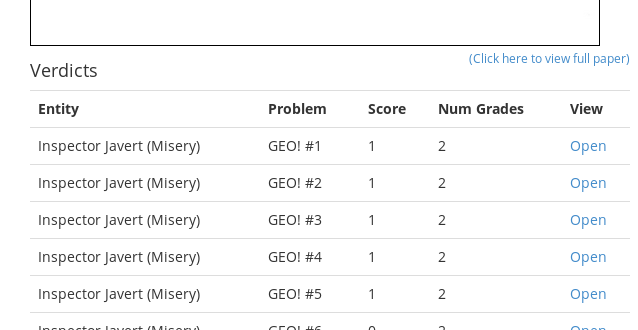
\includegraphics[width=0.6\textwidth]{images/viewpaper2.png}
\end{center}

If the paper has an exam scribble associated,
that will also be displayed,
along with a form to change the name associated to it
(in case of error).

\begin{center}
	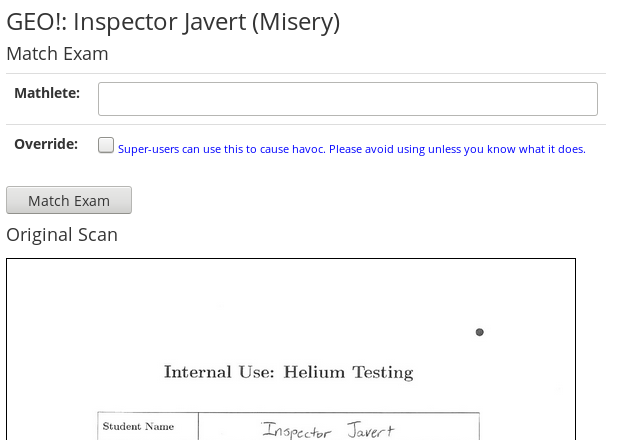
\includegraphics[width=0.6\textwidth]{images/viewpaper1.png}
\end{center}

\section{Conflict resolution}
First, I should describe the logic behind verdicts.
For each exam there are two parameters:
\begin{itemize}
	\ii A \textbf{minimum majority} for the verdict to be valid,
	defined as a constant $n$ such that an $n$-to-$1$ majority suffices.
	\ii If valid, a \textbf{minimum number of graders} needed before
	the verdict considers itself done.
	(So setting this number to $2$ is double-grading,
	$3$ is triple-grading, etc.\ and the default is $3$.)
\end{itemize}

Officers get an extra panel called ``View All Conflicts''.
This lets you see the grading conflicts for \emph{everyone}.

\begin{center}
	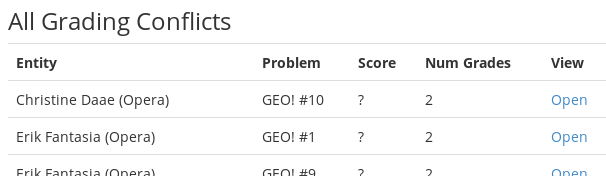
\includegraphics[width=0.8\textwidth]{images/all-conflict.png}
\end{center}

Given a conflict, you can open the verdict page corresponding to it,
at which point you can submit your own evidence.
If you like being final authority,
there should also be an option to submit this evidence in ``God mode''
which will settle the verdict once and for all.
\section{Finishing results}
Once grading is all said and done,
you can download the results at the bottom of the page.
Administrators can also download full results
and a full score spreadsheet.

Note that algorithmic scoring is not done automatically,
since it is a long and intensive operation.
To run it, you should use the management command
``Run Algorithmic Scoring'',
after all verdicts are settled.
Alternatively (and maybe better), you can use
\verb+python manage.py algscore+ from SSH.

\section{Other Administration}
The Django admin interface can be used if there
is some operation you need to do not supported by the existing views.

\subsection{Management}
In addition, to operations that might be useful
but in theory should not be necessary:
\begin{itemize}
	\ii ``Compute Verdicts'' will ask every verdict (and there will be many!)
	to re-compute its judgment.
	Normally, verdicts only re-compute their judgment when they get new evidence.
	This is needed if e.g.\ you change the thresholds for grading.

	\ii ``Update scribbles'' is similar,
	it updates all problem scribbles and verdicts
	with matched names.
	This should basically never be necessary unless you done goof.
\end{itemize}
Both of these commands actually just run \verb+manage.py+ commands,
so they can also be done from SSH.

\subsection{Someone uploaded PDF to wrong exam!}
Well, that's a bummer.  You should
\begin{itemize}
	\ii Delete the relevant PDF file from the Django admin interface.
	This will kill of the exam and problem scribbles too.
	\ii Delete all the verdicts that no have neither an entity or problem scribble.
\end{itemize}
That should mostly save things. No priomises though.

\chapter{Instructions for Helium administrator}
Here are some tasks you need to do to set up Helium
to work before the tournament, and after grading.

\section{Database maintenance}
\subsection{Rinse the database}
For posterity, first save another copy of the data using Django management:
\begin{center}
	\texttt{python manage.py dumpdata helium --indent 1}
\end{center}
This will output a file with all Helium related data.
Thus if you ever need it back you can then reload it with \texttt{loaddata}.

Then, one should SSH into the instance and run the following command.
\begin{center}
	\texttt{python manage.py helium\_rinse}
\end{center}
which will clear all Helium-related data.

\subsection{Import exams from Babbage}
You need to populate the Helium tables with exams.

To do this, you should go to the problem database and for each contest
that you want to export, push the ``Export to Helium'' link.
This will copy all the problems and their answers into Helium,
and then open the admin interface
so that you can make any manual changes necessary
(for example partial marks are disabled by default
but you will need to add them into Guts estimation).
Remember to input colors corresponding to how the answer sheets will be tinted.

A safety feature is that exam names in Helium must be distinct.
So if you decide you want to re-import an exam,
you will have to delete the old one first.

\subsection{Import entities from registration}
In Babbage a command called ``Import Entities from Reg'' will do this for you.
It is careful, and will never import the same entity twice.
This is also the ``heliumimport'' command.

It is very important to \textbf{run heliumimport as late as possible},
preferably just after the first individual exam begins.
Registration always changes last-minute.

\section{Guts estimation problems}
First, ensure that the name of the Guts exam is ``Guts'',
or otherwise maul \texttt{babbage/views.py} to make this work.

Next, if there are any estimation problems the scoring functions
for these need to be added.
You can do this in the admin interface, under ``Guts Score Funcs''.
This should be entirely self-explanatory.

\section{Printing and checking scans}
You should make sure that a large number of answer sheets are printed,
and in different colors between tests to avoid errors.

Unfortunately, right now the scan regions (i.e.\ the cut-outs)
are hard-coded into \verb+scanimage.py+.
So before the tournament you should check the scanners being used
and verify that the cut-out regions are compatible with the scanner.

The file \verb+scanimage.py+ has a facility to make this easier.
If you run
\begin{center}
\verb+python /path/to/scanimage.py FILENAME.pdf+
\end{center}
then it will generate (in the current directory)
the images corresponding to the cut-outs.
Thus you can test this locally and make adjustments to the regions if needed.
\section{Name stickers}
Make sure tournament directors are printing out name stickers for the students;
this will make grading life a lot easier.
Students should be instructed to:
place their name stickers in the field that says ``name'',
but still write their ID number in the blanks provided manually.

Also, on personalized schedules for teams, print out ID numbers.
Doing so will expedite the process of grading significantly.

This task takes place outside of Helium, and varies between tournaments.
The bottom line is that \textbf{ensure students and teams know their ID's}.

\section{Sanity checking results}
Once grading is done, you should do the following clean-up tasks.
\begin{itemize}
	\ii First, open the Verdict table in Django admin and look for verdicts which
	are ``inaccessible''.
	In theory there should be none.
	If such a verdict exists, do a sanity check to make sure it's an anomaly,
	then delete these verdicts.

	\ii If there are verdicts with no names, verify this is correct:
	these should only come about from no-name papers,
	or papers yet to be matched.

	In November 2016 for unknown reasons, some exam scribbles got matched
	but the underlying verdicts for them were left as None.
	You can auto-magically fix these by running the
	management command ``update scribbles''
	which will fix any issues.

	\ii Look in the Entity table for any entities which have
	no verdicts attached to them.
	First delete all individuals with no verdicts:
	this probably means that they did not show up.

	Teams can also not show up,
	but they can also leave early and not take Team or Guts round.
	That's why it's necessary to delete no-show individuals first.
	Only after this, if a team has no verdicts \emph{and} no individuals,
	then one can delete it.
\end{itemize}

\section{Last grading commands}
There are two different management commands at play.
You need to run both, in this order.

\begin{itemize} 
	\ii ``algscore'': this command is slow, taking about two minutes per run.
	It computes the $\alpha$ and $\beta$ values for each student
	based on the set of observations.

	\ii ``grade'': This command is fairly fast, it should take no more than
	a few seconds per run-through.
	It collates together all the results into a table which
	are then displayed in results reports.
	This is necessary because otherwise the process of aggregating the scores
	is too slow.
\end{itemize}

Run both commands, then look through the reports to make sure everything is okay.

It may be wise to run ``grade'' throughout the day,
just to make sure that things are looking okay.
The $\alpha$ and $\beta$ values won't be correct, but that's okay;
we don't need those values when we're just sanity checking results.
\section{Printing results}
The easy part.  After running the ``grade'' command,
the dashboard has several links to the scores in various formats
(OpenDocument spreadsheet, text file, etc),
and an automated awards presentation TeX file.
Congratulations on finishing!

\chapter{Notes for software team}
This contains low-level technical notes on some of the non-obvious
moving parts behind the whole system.
This is intended to help you extend Helium in some way.

Most of the code I tried to comment or \verb+help_text+ well.
But if anything is still confusing, that's probably my fault.
Feel free to contact me at \texttt{chen.evan6@gmail.com}.

\section{Personal request}
I have a personal request before you start editing,
which is that my name remains intact in \texttt{LICENSE.txt},
this documentation, and other places (for example file headers).
You are free of course to add your own name
should you make substantial contributions.

The reason I ask this is because this system represents
well over $200$ volunteered hours of my free time
pooled into over $400$ commits.
I built the entire system from scratch with no assistance from anyone else.
Since I didn't collect any payment for this work,
the least I ask is that I am recognized for it.

Thanks!

\section{A Warning}
I found out the hard way that a typical tournament has maybe $N = 30000$ verdicts in it.
This means you should make sure your code does not do either of the following per call:
\begin{itemize}
	\ii Do not use algorithms that run in $O(N^2)$ time.
	\ii Do not make $O(N)$ queries to the database.
\end{itemize}
For queries grabbing the entire verdicts table (or large portions of it),
it is almost always better to use the \texttt{queryset.values} method.
For these large values of $N$, creating $N$ instances from the table is just too slow.

\section{Test data}
\subsection{Location}
Some test data has been provided for you.
You can look for it in the following places:
\begin{itemize}
	\ii \verb+:/helium/static/batchX-samplescans.pdf+
	\ii \verb+:/helium/static/batchY-samplescans.pdf+
	\ii \verb+:/helium/fixtures/*+
\end{itemize}
The easiest thing to do is to load the two fixtures in the ``setup'' directory,
which will populate the exams and entities tables.
The sample scans correspond exactly to the entities in these fixtures.

You can also load fixtures in the \verb+:/helium/fixtures/scenarios+ directly
which are snapshots of the entire database at various points in time
in the test run
(after matching exams, after grading, after algorithmic scoring, etc.).
But note that the \verb+/media/+ folder is NOT included.

\emph{Warning}: the scenarios folder contains a superuser
with name and password ``evan''
as well as a staff user with name and password ``staff1''.
Consequently, be careful to NOT run these on production,
as we will then have some very insecure user accounts!

\subsection{Synopsis of test data}
Synopsis of test data:

\begin{itemize}
\ii There is a single scan-based exam, called ``GEO!'',
and there is a single non-scanned exam, called ``Mock IMO''.
The former is $10$ problems scored algorithmically.
The latter is $3$ problems worth $7$ points each.

\ii There are $16$ mathletes split into three teams of five,
corresponding to characters from \emph{L\'es Miserables},
\emph{Wicked}, and the \emph{Phantom of the Opera},
plus one unaffiliated individual named ``Evan Chen''.

\ii The two sample batches contain all their ``GEO!'' exams.
The answers to that exam corresponding exactly to the real answers
to the HMMT February 2016 Geometry test.

\ii Under the registration folder are some fixtures for testing
import to registration and so on.

\ii Under the problems folder are some fixtures for loading
some example data into the problem database.
\end{itemize}

\section{Moving parts}
When possible I tried to keep everything in Helium 
self-contained, not relying on even files outside the directory.

\subsection{Helium dependencies}
Here is a partial list of things externally that Helium relies on;
it may be incomplete.
All this is at time of writing;
other people move things around all the time so God knows
if we will even have \texttt{core/settings.py} in a few years.

\begin{itemize}
	\ii \texttt{requirements.txt} in the root directory
	has some Helium specific additions.
	In particular \texttt{wand} which does image processing in Python.
	The command
	\begin{center}
		\texttt{pip install -r requirements.txt}
	\end{center}
	should do the trick.

	\ii Image installation is done through the EB extension \texttt{01yum}.
	This installs \texttt{imagemagick}, \texttt{freetype}, \texttt{ghostscript},
	which is used for the image processing.

	\ii Helium needs to host its media on an external S3 server,
	because scan images need to be distributed.
	So currently I have an S3 bucket called \texttt{heliummedia}.
	The connection is in \texttt{core/settings.py},
	The S3 bucket itself lives inside AWS along with the entire HMMT application.
	
	\ii \texttt{core/settings.py} should also have some basic applications
	installed, such as
	\begin{itemize}
		\ii `django.contrib.admin',
		\ii `django.contrib.auth',
		\ii `django.contrib.sessions',
		\ii `django.contrib.messages',
		\ii `django.contrib.staticfiles',
		\ii `storages'.
	\end{itemize}
\end{itemize}

\subsection{Things depending on Helium}
\begin{itemize}
	\ii The Guts scoreboard reads its data from Helium.
	So if you make changes to Helium, check there too.
	
	\ii Registration import into Helium, as described before.
\end{itemize}

\subsection{Other nice things to know}
Some not terribly Helium-specific things, but you should still know:
\begin{itemize}
	\ii Logging configuration (not specific to Helium, but nice!)
	is done by the EB extension \texttt{00logging}
	and configured in \texttt{core/settings.py}.
	
	\ii Not Helium-specific, but the EB extension \texttt{05managepy}
	is responsible for running \texttt{collectstatic} and \texttt{migrate}.
\end{itemize}

\section{Git subtree}
There is an upstream URL which publishes Helium-specific code.
This way other math tournaments can use the same code themselves.

This upstream URL is maintained by a subtree via the command
\begin{center}
	\texttt{git subtree split --prefix=helium -b helium}
\end{center}
to create a branch \texttt{helium} containing only code from this folder.
Thereafter, we push this branch into the Git helium repository
(to the master branch on Git: note that the branch names differ).

The \texttt{README.txt} files provides a brief documentation
on how to get set up with Helium in a different Django project.

\section{A wishlist}
Some possible to-do things:
\begin{itemize}
	\ii Image processing: auto align scan regions and cut-outs.
	\ii Proof grading (long shot).
\end{itemize}


\appendix
\chapter{Terminology}
\label{ch:terms}

The grading system is itself known by the name \vocab{Helium}.
Each event will be referred to as a \vocab{contest}.

\section{Participants}
In each contest there are several participants.
The students are referred to as \vocab{mathletes}.
These students are often grouped into \vocab{teams}.
A mathlete may have no team; in this case we say they
are an \vocab{unaffiliated individual},
or sometimes just ``individual'' for short although this is confusing.

An \vocab{entity}\footnote{%
	This abstraction is useful because an exam doesn't care so much who takes it.}
refers to someone,
either a mathlete or a team,
who takes an exam.

A \vocab{user} refers to a staff member of the contest
(not a student or coach).
A \vocab{superuser} refers to a higher-level administrator of the contest;
for example a head grader, or problem czar,
or tournament director, or software director.
To be more exact this is the set of users with administrative
privileges on the Django website.

\section{Exams and problems}
A contest consists of several \vocab{exams}\footnote{%
	Helium deliberately avoids the word ``test'',
	since this may be confused with ``testing'' and so on},
each of which has several \vocab{problems},
which are numbered $1$, $2$, \dots, $n$ in each exam.
These exams are \vocab{taken} by entities,
who must attempt to solve the problems on the exam.

A problem has the following properties:
\begin{itemize}
	\ii The problem has a \vocab{weight},
	which is the number of points a contestant earns for solving it.

	\ii The problem may allow \vocab{partial} marks,
	or it may be an ``all-or-nothing'' problem.
\end{itemize}
Exams may be ``individual'' or ``team'' exams,
depending on which types of entities take them.

\section{Scans}
A \vocab{problem scribble} refers to the scan
of a contestant's answer to a problem.
An \vocab{exam scribble} refers to the scan
of a contestant's entire answer sheet for an exam.
You won't see these two terms much in the user interface,
but they are used internally in the source code just about everywhere.

A \vocab{paper} refers to the set of answers for
a contestant to any given exam,
regardless of whether the paper was fed into a scanner or not.

\section{Grading}
Suppose an entity $E$ attempts a problem $P$,
Helium then needs to give a \vocab{verdict} to the pair $(E,P)$,
which consists of a score assigned to the pair $(E,P)$.
This represents the judgment handed down by Helium to $E$
for this problem $P$.

To generate this verdict,
one or more users will input a score for the pair $(E,P)$.
Each such score by a grader is termed an \vocab{evidence}
contributing towards the verdict,
and we say the user \vocab{submits} this evidence.
The verdict is \vocab{valid} if there is a clear consensus what the final
score should be (by default this is at least a 3-to-1 majority,
but this may be adjusted per exam).
The verdict is \vocab{done} once it is valid and there is enough evidence.

There is one possible exception:
super-users may submit a evidence in \vocab{God mode}.
When this occurs, it overrides any and all evidence submitted by regular users.

\section{Algorithmic scoring}
At HMMT a complex algorithm is used for assigning
the weights to the individual tests.
Details of this algorithm are available at
\begin{quote}
	\url{https://www.hmmt.co/static/scoring-algorithm.pdf}
\end{quote}
A copy of this algorithm is also included in an appendix
at the end of this document.

Let $\mathcal A$ be the set of exams scored using this algorithm.
Each problem on an exam in $\mathcal A$
obtains a weight which is called a \vocab{beta value},
denoted $3 \le \beta \le 8$.
Moreover, each entity taking one or more exams in $\mathcal A$
is then assigned an \vocab{alpha value},
which represents their strength, and is denoted $\alpha \in \RR_{\ge 0}$.
These $\alpha$ and $\beta$ values are stored in database,
since they are quite hard to compute.

At HMMT the alpha values are used to aggregate individual scores
across all tests, and thus used to rank individuals.

\chapter{HMMT Algorithmic Scoring Details}
\section{Synopsis}
\subsection{Input}
Each exam contains at least one \textbf{problem}.
The exams are taken by several \textbf{contestants}.

This algorithm takes several \textbf{observations}:
i.e.\ it takes as inputs pairs $(c,p)$ of contestants and problems,
and for each such pair is told whether or not $c$ \textbf{solved} $p$.
During the actual tournament, every problem is attempted by every contestant;
however, the algorithm will not use this assumption.

\subsection{Output}
Based on this, the algorithm outputs:
\begin{itemize}
	\ii An \textbf{strength} $\alpha_c \in \RR_{\ge 0}$ for each competitor $c$, and
	\ii A \textbf{weight} $\beta_p \in [3,8]$ for each problem $p$,
	which represents its difficulty.
\end{itemize}
Note that the strength is \emph{not} the same as the score of a contestant.
In particular, as described below,
each contestant is given a single strength value across all exams.

\subsection{Usage in contest}
The calculation at the actual HMMT is done in one pass.
For example, at HMMT February 2016, there were three exams with $10$ problems
each and $700$ contestants.
Thus there were $700 \cdot 10 \cdot 3 = 21000$ observations as input.
Note that the algorithm is applied only once!
For example the observations on the Algebra test
affect the weights of the Geometry test.

For each particular 10-problem \textbf{exam},
the \textbf{score} of a contestant on that exam is the sum of the 
difficulties $\beta_p$ for each problem that they solve.
The score of a contestant is used to determine their rankings
within each individual test.
Scores across different exams are not comparable.

For individual sweepstakes, the strength $\alpha_c$ is used instead
(in order to ensure that no particular exam dominates
in determining the aggregate individual score).
Contestants are ranked based on the value of $\alpha_c$ assigned to them.
When determining team sweepstakes,
the individual contribution (out of $800$)
is proportional to the sum of $\alpha_c$ across the team members $c$,
scaled so that the strongest teams earns the maximal $800$ points.

\section{Design}
\subsection{Advantages}
The scoring algorithm is designed to meet the following criterion:
\begin{itemize}
	\ii The system provides a careful way to
	\textbf{compare scores across tests},
	leading to less noise in the aggregate individual
	and team rankings.

	\ii The system \textbf{factors all possible inputs},
	rather than for example merely the top 10 contestants or otherwise,
	as occurred in previous HMMT tournaments.

	\ii The system is \textbf{resistant to preconceived difficulty}.
	Originally, problem czars were forced to estimate the difficulty
	of every problem by assigning it a weight;
	this leads to possible noise in the results.
	The algorithmic system determines the difficulty based on the actual performance.

	\ii The system is \textbf{hard to exploit},
	in part because it takes inputs from all contestants,
	and in part because it is so complicated
	that a contestant is probably better off thinking about
	the exam problems.
\end{itemize}

\subsection{Qualitative criteria}
The following additional criteria are satisfied:
\begin{itemize}
	\ii The strength of each contestant is nonnegative,
	\ii The strength of a contestant is unbounded,
	but not infinite even if they solve every problem.
	\ii The strength of a contestant is zero
	if they solve no problems.
	\ii Problem weights lie in the interval $(3,8)$.
	\ii The distribution functions are smooth.
\end{itemize}

\subsection{Choice of priors}
In light of this, we select the following parameters,
which describe how the $\alpha_c$ and $\beta_p$ should be interpreted.
\begin{itemize}
	\ii The strength $\alpha = \alpha_c$ of each contestant
	$c$ is \emph{a priori} distributed in $\RR_{\ge 0}$
	according to
	\begin{equation}
		\mathbf P(\alpha) = \exp(-\alpha).
		\label{eq:cprior}
	\end{equation}
	\ii The weight (difficulty) $\beta = \beta_p$ of each problem $p$ is
	\emph{a priori} distributed in $[3,8]$ according to 
	\begin{equation}
		\mathbf P(\beta) = \exp\left( \frac{5}{(\beta-3)(8-\beta)} \right).
		\label{eq:wprior}
	\end{equation}
\end{itemize}
Now we relate the strength $\alpha = \alpha_c$ of contestant $c$
to the difficulty $\beta = \beta_p$ of problem $p$ by
postulating that the probability that $c$ solves $p$ is
\begin{equation}
	\mathbf P
	\left( \text{$c$ solves $p$} 
	\mid \alpha_c = \alpha \text{ and } \beta_p = \beta \right)
	= \frac{\exp(-\beta/\alpha)}{1 + \exp(-\beta/\alpha)}.
	\label{eq:prob}
\end{equation}
Assuming \eqref{eq:cprior}, \eqref{eq:wprior}, \eqref{eq:prob}
and holding fixed the set of observations of the tournament:
\begin{quote}
\itshape
The algorithm outputs the unique set of $\alpha_c$ and $\beta_p$
for which the outcome of the tournament was most likely.
\end{quote}
The rest of the document describes how to actually compute
the maximum.

\section{Algorithm Description}
The algorithm is a slightly modified version of the Rasch model.

\subsection{Pseudocode}
Let us for brevity denote the function in \eqref{eq:prob} by 
\[ w(\alpha, \beta) \defeq \frac{\exp(-\beta/\alpha)}{1 + \exp(-\beta/\alpha)}. \]
Note that $w(\alpha, \beta) \in (0,1)$,

Now consider the following systems of equations,
whose origin we explain below.
First, for every $\alpha = \alpha_c$ we have the equation
\begin{equation}
	0 = -1 + \sum_{\text{$p$ solved by $c$}} \beta_p\alpha^{-2}
		- \sum_{\text{$p$ took by $c$}} \beta_p \alpha^{-2} w(\alpha, \beta_p).
	\label{eq:alpha}
\end{equation}
Moreover, for every $\beta = \beta_p$ we have the equation
\begin{equation}
	0 = \frac{1}{(\beta-3)^2} - \frac{1}{(8-\beta)^2}
		+ \sum_{\text{$c$ taken by $p$}} \alpha_c^{-1} w(\alpha_c, \beta)
		- \sum_{\text{$c$ solved by $p$}} \alpha_c\inv.
	\label{eq:beta}
\end{equation}
The algorithm binary searches for a set of $\vec\alpha$ and $\vec\beta$
which simultaneously satisfy \eqref{eq:alpha} and \eqref{eq:beta}.
It is proved below that this set of parameters is unique;
this is the output of the algorithm.


\subsection{Derivation}
We show the derivation of equations \eqref{eq:alpha} and \eqref{eq:beta}.

Fix a set of observations for the tournament.
Now consider a choice of $\vec\alpha$ and $\vec\beta$ is known.
Then the probability of the observations is distributed according to
\begin{equation}
	F( \vec\alpha, \vec\beta )
	= \prod_{c} \mathbf P(\alpha_c)
	\prod_{p} \mathbf P(\beta_p)
	\prod_{\text{$c$ solved $p$}} w(\alpha_c, \beta_p)
	\prod_{\text{$c$ missed $p$}} (1-w(\alpha_c, \beta_p))
	\label{eq:F}
\end{equation}
assuming the events are independent.

We now claim that:
\begin{proposition}
	If a choice of $\vec\alpha$ and $\vec\beta$ optimizes $F$,
	then it is a solution to \eqref{eq:alpha} and \eqref{eq:beta}.
	In other words, the outputted $\vec\alpha$ and $\vec\beta$
	are those for which the observed outcome was most probable.
\end{proposition}

\begin{proof}
	Note that
	\[
		\prod_{\text{$c$ solved $p$}} w(\alpha_c, \beta_p)
		\prod_{\text{$c$ missed $p$}} (1-w(\alpha_c, \beta_p))
		=
		\prod_{\text{$c$ solved $p$}} e^{-\beta_p/\alpha_c}
		\prod_{\text{$c$ took $p$}} \frac{1}{1+e^{-\beta_p/\alpha_c}}.
	\]
	From this, and plugging in \eqref{eq:cprior} and \eqref{eq:wprior}, we get
	\[
		F(\vec\alpha, \vec\beta)
		= \prod_{c} e^{-\alpha_c}
		\prod_{p} e^{-\frac{5}{(8-\beta_p)(\beta_p-3)}}
		\prod_{\text{$c$ solved $p$}} e^{-\beta_p/\alpha_c}
		\prod_{\text{$c$ took $p$}} \frac{1}{1+e^{-\beta_p/\alpha_c}}.
	\]
	It is equivalent to maximize $\log F$, which is
	\[
		\log F
		= -\sum_{c} \alpha_c
		- \sum_{p} \frac{5}{(8-\beta_p)(\beta_p-3)}
		- \sum_{\text{$c$ solved $p$}} \frac{\beta_p}{\alpha_c}
		+ \sum_{\text{$c$ took $p$}} \log\frac{1}{1+e^{-\beta_p/\alpha_c}}.
	\]
	Then right-hand sides of \eqref{eq:alpha} and \eqref{eq:beta}
	are the \emph{partial derivatives} of $\log F$ with respect
	to $\alpha_c$ and $\beta_p$ for each $c$ and $p$.
	The partial derivatives equal zero at any local maximum of $\log F$,
	as desired.
\end{proof}

In fact, one can actually check that the right-hand sides of 
\eqref{eq:alpha} and \eqref{eq:beta}
are monotonic in $\alpha$ and $\beta$ respectively.
Consequently, $F$ is convex.
This implies:
\begin{proposition}
	The function $\log F$ has a unique point at which all partial
	derivatives vanish, and that point is a maximum for $F$.
\end{proposition}

This also implies that one can numerically solve the equations
by the following binary search procedure.
We let $\vec\alpha_0$ be an arbitrary point.
Then we let $\vec\beta_n$ be the solution to \eqref{eq:beta} given $\vec\alpha_{n-1}$.
Notice that one can actually solve for each component $\beta_p$
using binary search separately,
as each equation of the form \eqref{eq:beta} involves only a single $\beta_p$.
Similarly, we can let $\vec\alpha_n$ be the solution to \eqref{eq:alpha}
given $\vec\beta_{n-1}$ in the same fashion.
The pairs $(\vec\alpha_n, \vec\beta_n)$ will converge to the maximum
since we are looking at partial derivatives of a concave function,
so we now have an iterative procedure for computing the output.


\end{document}
